%!TEX root = ../../Master.tex
\section{Analogue Navigation in Hospitals} % (fold 
\label{sec:anal_nav}

This section discusses existing analogue navigation platforms in order to draw experience from these. Strengths and weaknesses are analysed, providing a solid base for advancements in hospital navigation to be made in this report. A major source of information for this section is a trip to Sygehus Nord in Aalborg. The reason for the visit to Sygehus Nord was to examine navigation aid at a hospital.

Some figures in this section, were taken during the research at Sygehus Nord. Some assumptions made in \cref{sec:anal_nav} are based on the field research.

\subsection{Signs} \label{sub:sign}
Signs are usally used to mark key areas of a hospital. An example of a hospital sign could be \enquote{Main entrance} and \enquote{Ambulance entrance} \cite{signs_hospital,art_Osborne}.

Interior signs are typically affixed to walls, doors, windows or hung from the ceiling. Signs serve different purposes; they can display the name of a location or mark the general direction of one. See \cref{fig:signs1,fig:signs2}.

Signs are good at guiding users because of their directional properties and their ability to provide relevant information for key positions. On the other hand, signs can be hard to spot if the visitor is not familiar with hospitals. Sign can be visually obstructed, for example covered by other signs. Another problem regarding signs, is that they expect the visitor to be literate. This is a problem for foreigners who do not understand the language or other illiterates \cite{signs_reading}. Overflow of information displayed on signs can confuse the user. This is due to the fact that signs displays general information, and thus does not only cater to individual needs. Sign are of no use for people with a major visual impairment.


\begin{figure}
\centering
  \begin{minipage}{0.45\textwidth}
    \centering
    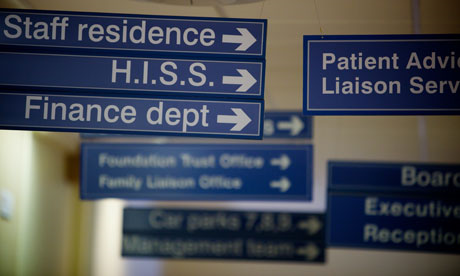
\includegraphics[width=\textwidth]{Alder-Hey-hospital-signs-007.png}
    \caption{Signs placed along a hallway \cite{signs_hospital}.} \label{fig:signs1}
  \end{minipage}
  \hfill
  \begin{minipage}{0.45\textwidth}
    \centering
    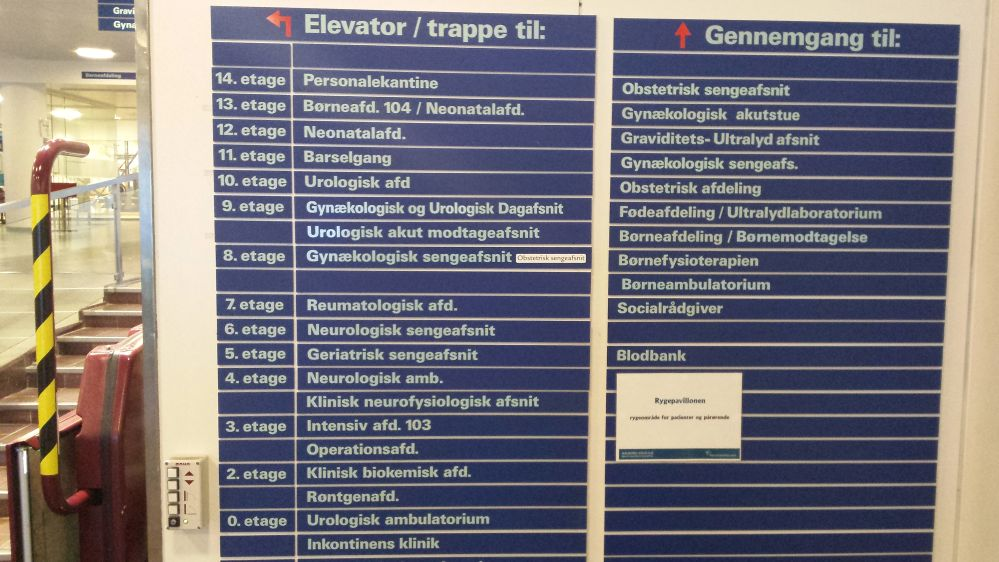
\includegraphics[width=\textwidth]{tavle.jpg}
    \caption{An overview sign of the different floors at Sygehus nord Aalborg} \label{fig:signs2}
  \end{minipage}
  \end{figure}

\subsection{Maps} \label{sub:map}
Analogue maps \cite{map} offer a top-down view of the hospital with locations marked by text or colour \cite{art_Osborne}. See \cref{fig:map}. Maps can be affixed to walls or made in compact versions meant for carrying. Stationary maps may have a mark, showing the location of the map. By knowing the current position, the visitor's ability to navigate should improve as they will not have to survey their surroundings for recognizable objects identifying their position \cite{map_survey}. In case the building has multiple floors, the map will be split up into layers each depicting a floor in order to more easily represent a 3D structure.

Maps are able to show areas of interest and quickly give an overview of the location in a manageable way \cite{pros_analog_map}. However this is not always the case, since maps complexity is greatly increased when covering large areas or multiple floors \cite{map_confusing}. If the visitor is already inside the building, it can be difficult to figure out where they are corresponding to the map. If the visitors are in a hallway it can be difficult to distinguish it from other hallways on the map.

  \begin{figure}[ht!]
  \centering
  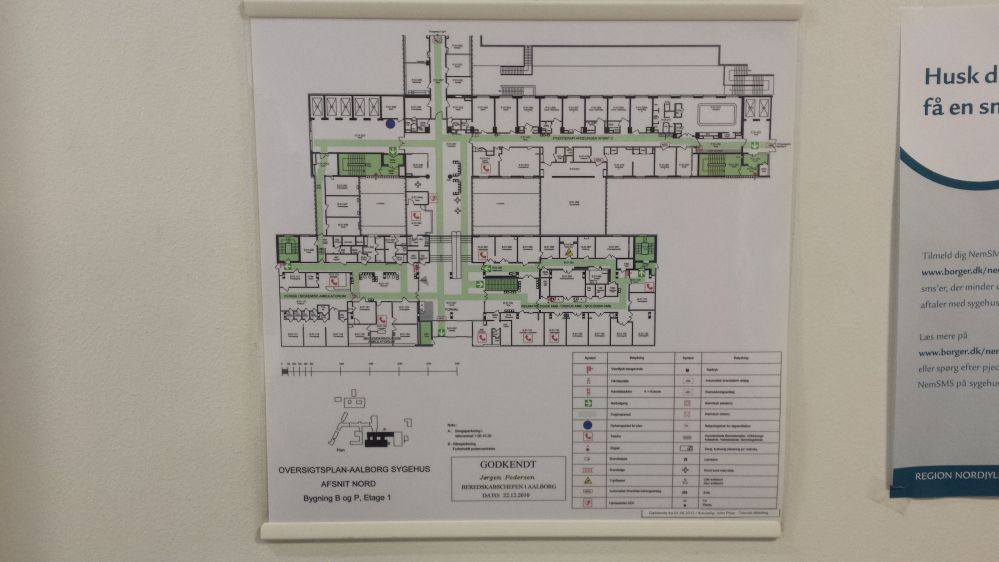
\includegraphics[width=90mm]{kortvaeg.jpg}
  \caption{A map on a wall at Sygehus nord Aalborg}
  \label{fig:map}
  \end{figure}

\subsection{Colour Coding}\label{sub:col}
Colour coding in hospitals are typically coloured lines painted on the walls or floors. See \cref{fig:colour_floor}. They mark key routes to certain locations in the hospital, that is usually displayed by a accommodating sign. Some areas may also have a dedicated colour theme. This makes it easier for users to navigate the hospital, by the colour representing the area.
Hospitals that use this method of navigation would seamlessly offer an easy way of letting the visitors navigate, because the information provided by the colours is simple to understand.

A problem with colour coding is the static nature of it. Changes to the infrastructure, could require repainting the walls and floors of the hospitals. Lines leading to many different areas, could potentially clutter up and become confusing. This method also does not provide guidance to visually impaired people.

\begin{figure}[htb]
  \begin{center} 
    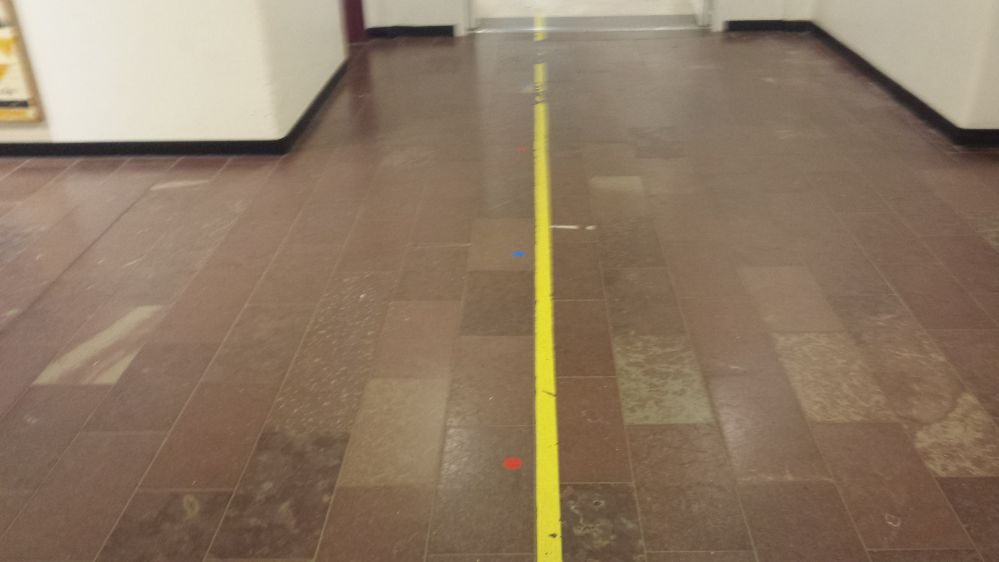
\includegraphics[width=0.5\textwidth]{stribe2.jpg}
  \end{center}
  \caption{Colour coding in use at Sygehus nord Aalborg}
  \label{fig:colour_floor}
\end{figure}

\subsection{Telecommunication}\label{sub:pho}

Visitors are able to call the hospital main number with various questions, such as navigation issues \cite{sign_ring}. Because the operator is in direct contact with the user, the information given will be specific. It is also easier for the user to come with follow up questions, as both parties are in a dialogue.
 
The limitations of this navigation method are many due to shortcomings of verbal assistance, which can often cause miscommunication. This method of navigation depends strictly on the operator assigned to answer the phone. If no one is at the phone, this method becomes impossible.
If the service is used in infrequent times of the day, assigning operators can prove difficult. If the phone is constantly in use, a queue will cause inconvenience for the users. If not, operators will experience standby time, which is inefficient use of resources.

\subsection{Personnel Interaction}\label{sub:human}
Visitors can ask hospital personnel regarding hospital navigation \cite{job}. This is similar to the telecommunication, but with the advantage of using body language, when answering the question \cite{body_vs_phone}.

At \enquote{Sygehus Nord Aalborg} a reception is located at the main entrance. See \cref{fig:rec_booth}. If a visitor arrives at an entrance different from the main one, they might not know where the reception is. The information received from the receptions has to be memorized by the visitor. This could prove problematic for some users. To overcome this problem, receptionists could write down instructions. These could still be misinterpreted due to different issues, such as crudeness or incorrectness.

  \begin{figure}[ht!]
    \centering
    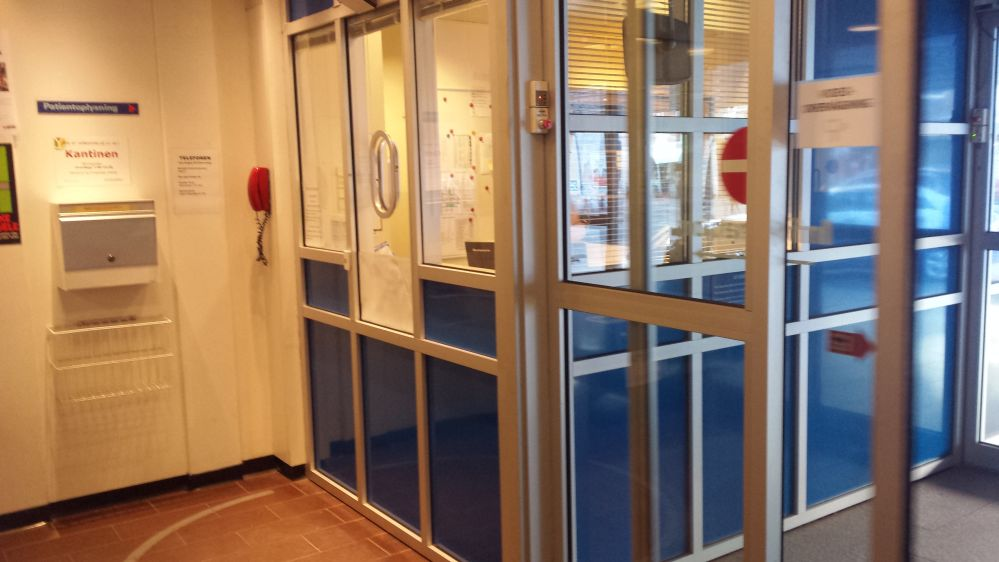
\includegraphics[width=90mm]{reception.jpg}
    \caption{A reception at Sygehus nord Aalborg}
    \label{fig:rec_booth}
  \end{figure}

\subsection{Summary} % (fold)
  In order to have a good navigation platform, the platform needs to be; easy to interpret (\cref{sub:sign}), give a quick overview (\cref{sub:map}), be precise (\cref{sub:human}), and easy to understand (\cref{sub:col}). The design of a solution has to avoid the weaknesses discovered in \cref{sec:anal_nav}. A solution must; not display irrelevant information (\cref{sub:sign}), deal with the representation of multiple floors in a clear way (\cref{sub:map}), deal with positioning without user interaction (\cref{sub:map}), be easy to maintain (\cref{sub:pho}).